\documentclass[12pt, utf8, ngerman, notes]{beamer}

\include{rvs}

\usepackage{pgfpages}
\usepackage{minted}
\usepackage{booktabs}
%\setbeameroption{show notes on second screen=right}

\title{Zitierungsanalyse mit Kylin}
\subtitle{Big OLAP: Data-Warehouse}
\author{Sebastian Lange, Simon Hüning, Klemens Schölhorn}
\date{04.03.2016}

\usetikzlibrary{arrows}
\usetikzlibrary{positioning}
\usetikzlibrary{matrix}

\begin{document}

% Titlepage
{
    \setbeamertemplate{footline}[default]
    \begin{frame}
        \titlepage
    \end{frame}
}

\begin{frame}{Einleitung und Aufgabenstellung}
  Data-Warehouse (DWH)
  \begin{itemize}
    \item Analyseabfragen
    \item Star-Schema
    \begin{itemize}
      \item \textbf{Faktentabelle} Messwerten, Kennzahlen, ...
      \item \textbf{Dimensionstabellen} Beschreibenende Daten (Autorenname, Buchtitel, ..)
    \end{itemize}
    \item OLAP-Würfel
  \end{itemize}
  Aufgabenstellung
  \begin{itemize}
    \item Analyse des Ausgangsdatensatzes
    \begin{itemize}
      \item DBLP - Sammlung wissenschaftlicher Publikationen
    \end{itemize}
    \item Importierung in das HDFS
    \item Transformation des Datensatzes in das Star-Schema
    \item Erzeugung der OLAP-Würfel
    \item Vergleich Kylin-Anfragen/HQL-Anfragen
  \end{itemize}
 \end{frame}
\note[itemize]
{
	\item Ein Data Warehouse (DW oder DWH) ist eine für Analysezwecke optimierte zentrale Datenbank, die Daten aus mehreren, in der Regel heterogenen Quellen zusammenführt und verdichtet.
    \item Faktentabelle - Foreignkeys + Fakten
    \item Dimensionstabelle - Beschreibene Daten, Name, Alter, etc...
    \item Innerhalb wissenschaftlicher Arbeiten werden andere Arbeiten zitiert
    \item Anzahl der Zitierungen charakterisiert wissenschaftlichen Einfluss
}

\begin{frame}{Verwendete Technologien}
  \begin{itemize}
    \item Hadoop 2.7.1
    \item HBase 0.98.15 (Hadoop 2.2 Bibliotheken)
    \item Hive 0.14.0
    \item Kylin 1.2
    \item Flink 0.10.1 (Hadoop 2.7 Bibliotheken)
    \item MySQL 5.5.47 (Hive-Metastore)
  \end{itemize}
\end{frame}
\note[itemize]
{
	\item Hadoop/HDFS - MapReduce-Framework/verteiltes Dateisystem - single node setup
    \item HBase - Key/Value-Store
    \item Hive - DWH-Erweiterung für Hadoop mit eigener Abfragesprache (HQL)
    \item Kylin - OLAP-Engine
    \item Flink - Hadoop-ETL-Framework
}

\begin{frame}{Datenfluss}
	\begin{tikzpicture}[auto]
        \node (dblp) {\includegraphics[width=3cm]{logo/dblp}};
        \node (hdfs) [right = 4cm of dblp]{\includegraphics[width=3cm]{logo/hdfs}};
        \node (hive) [below = 3.5cm of hdfs] {\includegraphics[width=2cm]{logo/hive}};
        \node (hbase) [left = 4.3cm of hive] {\includegraphics[width=3cm]{logo/hbase}};
        \node (analyse) [below right = .8cm and -.5cm of dblp] {\Huge\textcolor{rvs-darkred}{\textbf{Analyse}}};
        \draw<1>[-latex'] (dblp) to node {\includegraphics[width=2.7cm]{logo/pentaho}} (hdfs);
        \draw<2->[-latex'] (dblp) to node {\texttt{pub-importer}} (hdfs);
        \draw<1-2>[-latex'] (hdfs) to[out=250,in=110] node[align=left,pos=.4] {\includegraphics[width=2.7cm]{logo/pentaho}} (hive);
        \draw<3>[-latex'] (hdfs) to[out=250,in=110] node[align=left,pos=.2] {\includegraphics[width=2cm]{logo/flink}\\\texttt{pub-formatter}} (hive);
        \draw[-latex'] (hive) to node [above=.1cm,pos=.7,align=center] {\includegraphics[width=1.5cm]{logo/kylin}\\Kylin} (hbase);
        \draw[-latex'] (hbase) to (analyse);
        \draw[-latex'] (hive) to (analyse);
    \end{tikzpicture}
\end{frame}

\begin{frame}[fragile]{Import: \texttt{pub-importer}}
\begin{minted}[fontsize=\scriptsize]{xml}
<article mdate="2012-09-16" key="journals/tkde/FanS93a">
    <author>Jang-Jong Fan</author>
    <author>Keh-Yih Su</author>
    <title>Corrections to "An Efficient Algorithm
           for Matching Multiple Patterns".</title>
    <year>1993</year>
    <volume>5</volume>
    <journal>IEEE Trans. Knowl. Data Eng.</journal>
    <number>5</number>
    <url>db/journals/tkde/tkde5.html#FanS93a</url>
    <cite>journals/tkde/FanS93</cite>
</article>
\end{minted}
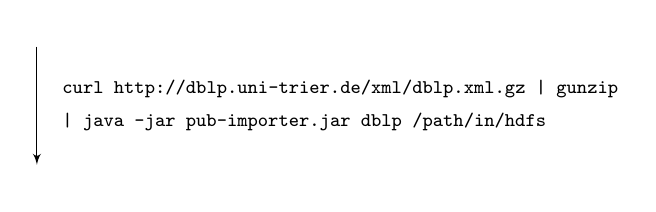
\begin{tikzpicture}
	\node (t1) {};
    \node (t2) [below = 1.5cm of t1] {};
    \draw[-latex'] (t1) to node[align=left,right=.2cm] {\scriptsize\texttt{curl http://dblp.uni-trier.de/xml/dblp.xml.gz | gunzip}\\\scriptsize\texttt{| java -jar pub-importer.jar dblp /path/in/hdfs}} (t2);
\end{tikzpicture}
\begin{minted}[fontsize=\scriptsize]{xml}
7802,article,journals/tkde/FanS93a,Corrections to "An Efficient
Algorithm for Matching Multiple Patterns".,1993,IEEE Trans. Knowl.
Data Eng.#5#5,Jang-Jong Fan|Keh-Yih Su,journals/tkde/FanS93
\end{minted}
\end{frame}

\begin{frame}{Transformation: \texttt{pub-formatter}}
\begin{columns}
      \column{\dimexpr\paperwidth}
      \begin{figure}[H]
          \begin{center}
              \includegraphics[width=\paperwidth]{pics/Star-Schema.png}
          \end{center}
      \end{figure}
	\end{columns}
\end{frame}

\begin{frame}{Transformation: \texttt{pub-formatter}}
\begin{columns}
      \column{\dimexpr\paperwidth}
      \begin{figure}[H]
          \begin{center}
              \includegraphics[width=\paperwidth]{pics/Star-Schema-final.png}
          \end{center}
      \end{figure}
	\end{columns}
\end{frame}

\begin{frame}{Analyse: Kylin}
	\begin{columns}
      \column{\dimexpr\paperwidth}
      \begin{figure}[H]
          \begin{center}
              \includegraphics[width=\paperwidth]{pics/kylin_diagram.png}
          \end{center}
      \end{figure}
	\end{columns}
\end{frame}
\note[itemize]
{
	\item MOLAP für Hadoop
    \item Nutzung von HBASE für Cube Generierung
    \item SQL Engine (Apache Calcite)
	\item Adhoc-Analyse
}

\begin{frame}{Probleme und Einschränkungen}
	\begin{itemize}
        \item Pentaho Data Integration
        \begin{itemize}
            \item StAX Parser schlecht integriert
            \item JOINs komplett in Zwischenspeicher
            \item Performance Probleme bei kompletter Datenmenge \\
            (12 GB RAM nicht genug)
            \item Umständliche Konfiguration für Nutzung auf Cluster
        \end{itemize}
        \item Flink
        \begin{itemize}
			\item Kein standardkonformer CSV-Reader
        \end{itemize}
        \item Hive
        \begin{itemize}
            \item Inkorrekte Speicherberechnungen (alte Version)
        \end{itemize}
        \item Kylin
        \begin{itemize}
			\item Keine VIEW als Lookup-Table verwendbar
            \item SQL Engine hat Probleme mit DISTINCT
		\end{itemize}
    \end{itemize}
\end{frame}

\begin{frame}{Ergebnisse}
	\footnotesize
    \centering
	\begin{tabular}{lr|r|r}
        %\textbf{Abfragen} & \multicolumn{3}{c}{\textbf{Ausführungszeit (in Sekunden)}} \\\hline
                          & \textbf{HIVE} & \textbf{KYLIN} & \textbf{Ersparnis} \\\cmidrule[1.2pt]{2-4}
        \# Pub/Autor      &      177,34 s &        51,33 s & \textbf{126,01 s} \\\midrule
        \# Pub/Autor/2015 &       76,88 s &         7,55 s &  \textbf{69,33 s} \\\midrule
        max Zit/Autor/Pub &      120,73 s &        15,37 s & \textbf{105,36 s} \\\midrule
        max Zit/Autor     &      317,96 s &        31,80 s & \textbf{286,16 s} \\
        \midrule[1.2pt]
        \# Pub/Rahm       &       70,70 s &         0,07 s &  \textbf{70,63 s} \\\midrule
        \# Pub/Rahm/2015  &       59,76 s &         3,71 s &  \textbf{56,05 s} \\\midrule
        max Zit/Pub/Rahm  &      184,85 s &         0,32 s & \textbf{184,53 s} \\\midrule
        sum Zit/Rahm      &       58,63 s &         4,79 s &  \textbf{53,84 s} \\
        \midrule[1.2pt]
        \# Pub/Groß       &       94,35 s &         0,13 s &  \textbf{94,22 s} \\\midrule
        \# Pub/Groß/2015  &       79,25 s &         0,08 s &  \textbf{79,17 s} \\
        \midrule[1.2pt]
        \textbf{Mittelwert} &    124,05 s &        11,52 s & \textbf{112,53 s}
    \end{tabular}
\end{frame}

\begin{frame}{Ergebnisse}
\begin{columns}
      \column{\dimexpr\paperwidth}
      \begin{figure}[H]
          \begin{center}
              \includegraphics[width=\paperwidth]{pics/bigprak_dia.png}
          \end{center}
      \end{figure}
	\end{columns}
\end{frame}

\end{document}
